\section{辅助说明}

\subsection{运行方式}

\subsection{截图}

\begin{figure}[h!]
    \centering
    \begin{subfigure}{0.45\textwidth}
        \centering
        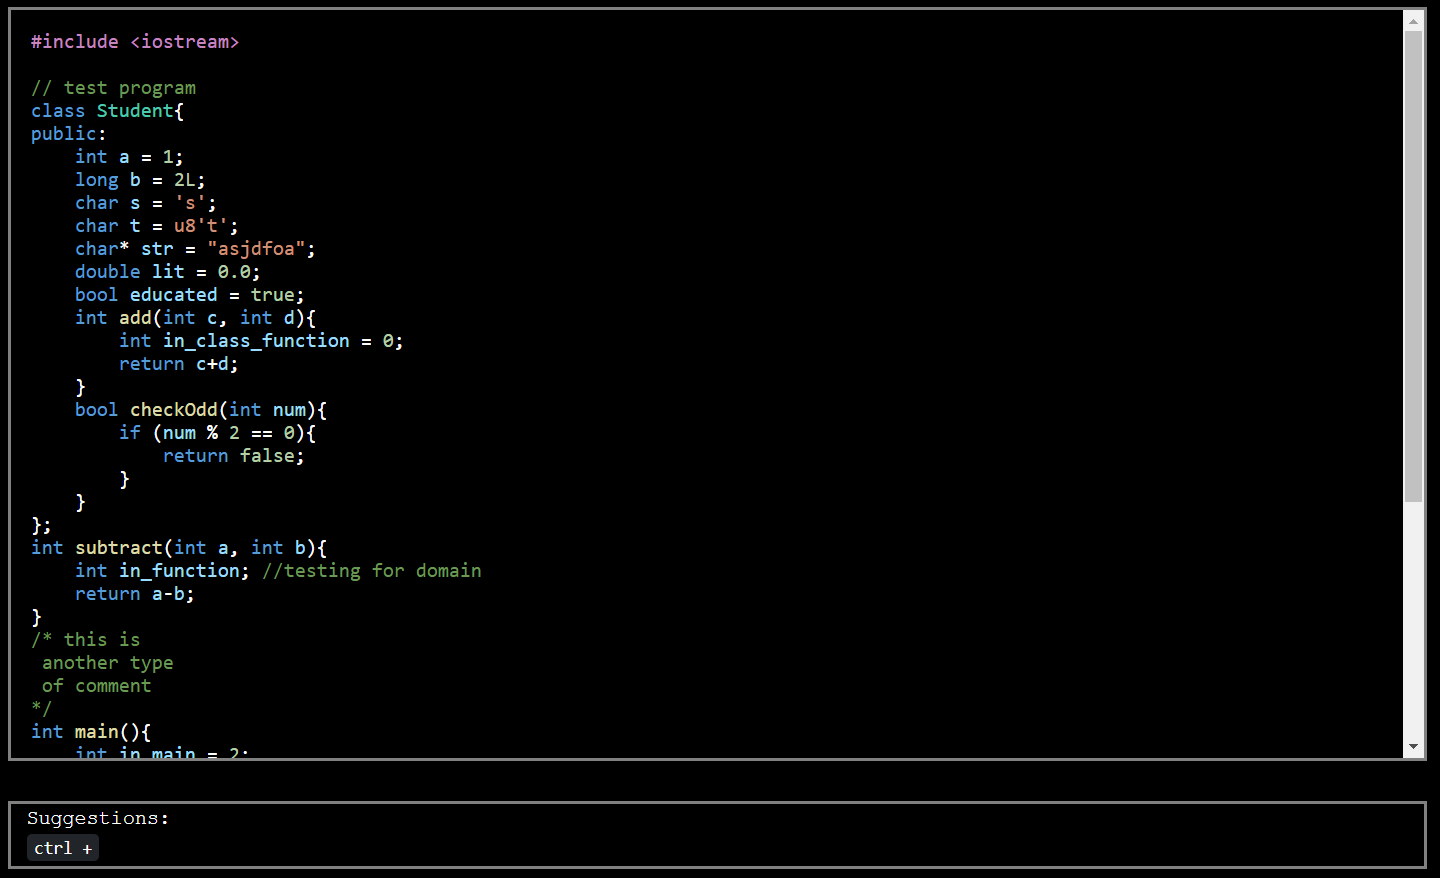
\includegraphics[width=\linewidth]{imgs/整体的样子.png}
        \caption{整体的样子}
        \label{fig:1}
    \end{subfigure}
    \hspace{1em}
    \begin{subfigure}{0.45\linewidth}
        \centering
        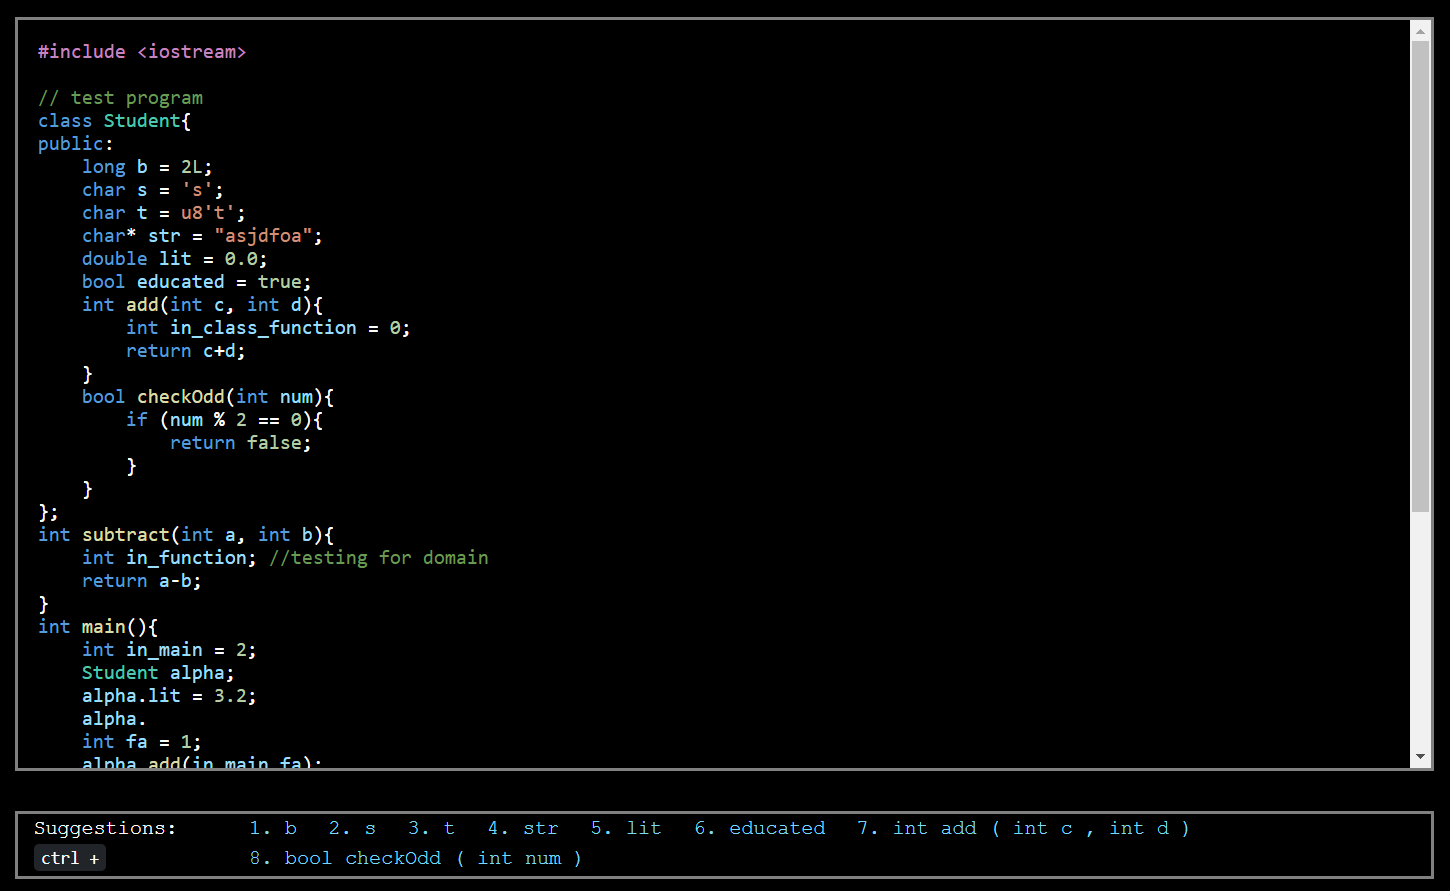
\includegraphics[width=\linewidth]{imgs/类成员对象和成员函数补全.png}
        \caption{类成员对象和成员函数补全}
        \label{fig:2}
    \end{subfigure}
    \begin{subfigure}{0.45\textwidth}
        \centering
        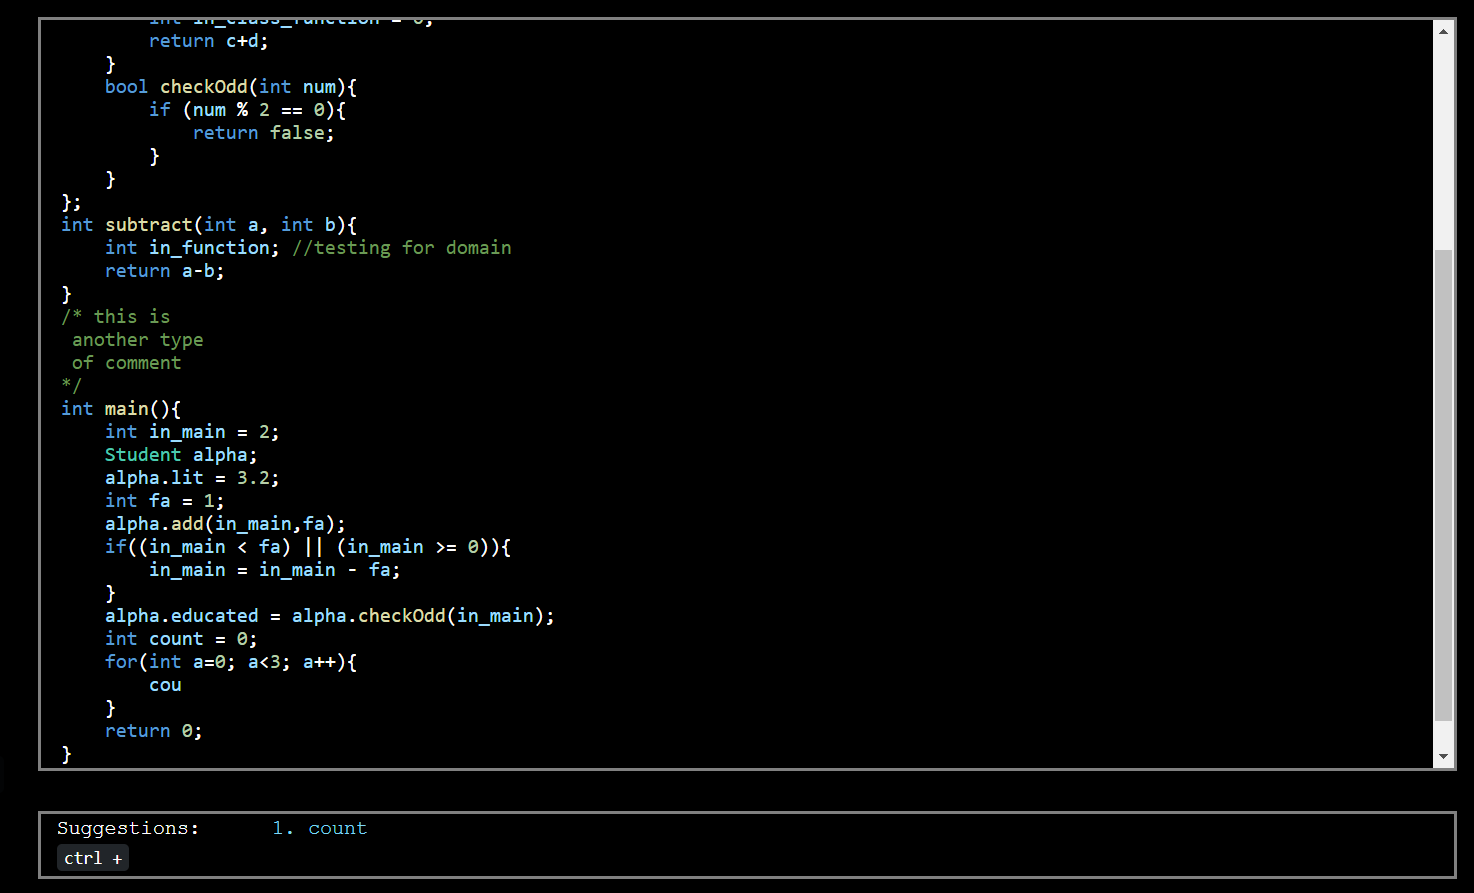
\includegraphics[width=\linewidth]{imgs/定义域内变量补全.png}
        \caption{定义域内变量补全}
        \label{fig:3}
    \end{subfigure}
    \hspace{1em}
    \begin{subfigure}{0.45\linewidth}
        \centering
        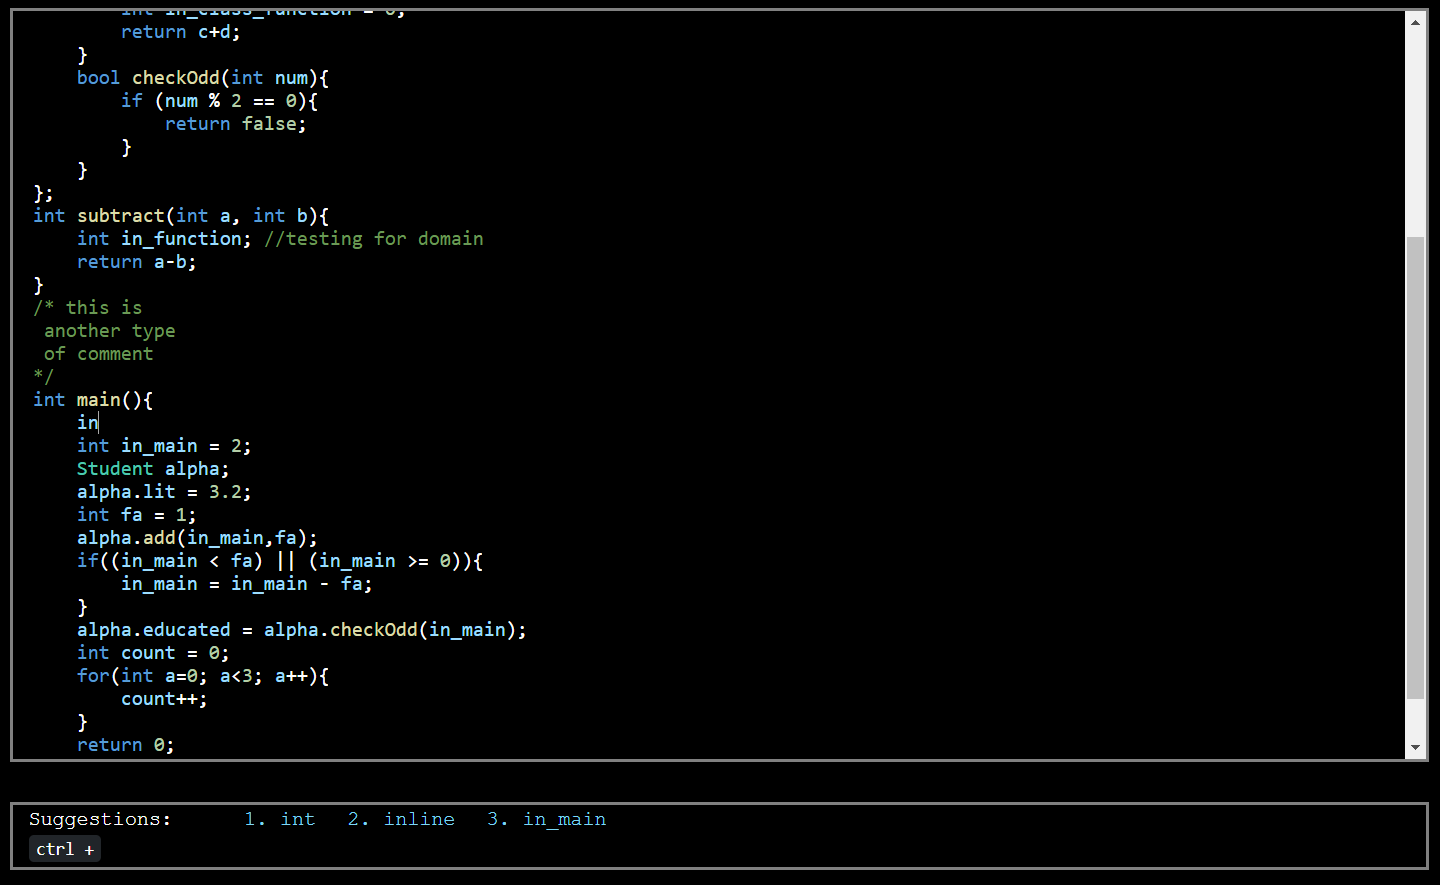
\includegraphics[width=\linewidth]{imgs/非定义域内变量(in_function)不补全.png}
        \caption{非定义域内变量不补全}
        \label{fig:4}
    \end{subfigure}
    \caption{代码高亮与提示程序截图}
\end{figure}

